\chapter{Organisation}

\section{Planning}
% What i did, when, how long
TODO

\subsection{Gantt}
% Disovering the team, the PWF
% Working with them within the scrum: xml stories
%

\section{Agile methodology}

In the team I was working, we were organized around Agile software
development. This way of working promotes incremental results and adaptive planning.
There are several implementations of Agile methods. In our team we were using Scrum.

In order to understand how I worked during my internship, some key concepts of Scrum must be described.

\subsection{Core concepts}

\subsubsection{Story}\label{sec:story}
A story is a \emph{business-oriented}, short description of a client's
need. Most of the times, it is divided into several tasks so that the developers
can take small steps to complete the story. A story is usually printed or
written on sticky note. Those notes are grouped on a story board.

\begin{figureGraphics}{A story board}{fig:storyboard}
    TODO picture of a story board
\end{figureGraphics}


\subsubsection{Sprints}\label{sec:sprint}
Sprints are short development cycles, usually from one to four weeks. We were
delivering results every three weeks. During each sprint, a team creates a
shippable product, no matter how basic that product is. A sprint is composed of
a set of stories which should be completed at it's end.

The interesting part of working in sprints is the idea of "making a fresh start" every three weeks. This
was quite motivating to me!


\subsection{Team}
Our team is composed of six members(me included); all software engineers with various
skills. Some are more software design oriented while others are more hardware
specialists.

In a Scrum, some members have a particular role:
\begin{description}
    \item[The Product owner]
        defines what the team is doing during a Sprint (see \ref{sec:sprint}).
        He determines the priority of each story (see \ref{sec:story}) the team is working on. His input usually comes from
        clients. He is the business-oriented person in the team. His decisions have an impact on the results a Scrum team delivers.
    \item[The Scrum master]
        ensures that every team member is correctly focused on his story. He is keeping track of the progress of each member and
        should alert the Product owner when some planning issues occur (bad time estimation, very urgent incoming task, ...).
\end{description}

Note that in our team, the Product owner and the Scrum master were also contributing to the team as software engineers.

\subsection{Events}
In Scrum, there are several events occurring during a sprint.
These are essential to the scrum methodology.

\subsubsection{Daily scrum}
Every day, at 11:30 we were holding the daily scrum meeting, also called "stand-up".
During that time, each member of the team answers quickly the three following questions:

\begin{description}
    \item[What have I done since yesterday ?]
    \item[What am I planning for today ?]
    \item[Any issues encountered ?]
\end{description}

This meeting is very useful, it helps tackle early problems and can assist the scrum master to detect delays in delivering.
Note that this should not take longer than 15 minutes.


\subsubsection{Poker planning}
TODO


\subsubsection{Demos}
At the end of each sprint, the team has to demonstrate their achievements. This
is a very important meeting with people external to the team. Only the work
which was \emph{completely done} during the last sprint is showed off during that presentation.
This presentation is about one hour. It is important to focus on the business value of the things that
have been done during the last sprint and set apart the technical details.  TODO reword a bit

\subsubsection{Retrospectives}
After the Demo, the team has a look back at how the last sprint happened. This short meeting is made
to find out what the team did wrong last sprint, but also to highlight what the team did right!
It is frequent to see little psychological games during the retrospective, which makes all members more
eager to participate.

\section{Workflow}
In this section, we will see 
TODO

\subsection{Setup}
Since compiling the Android source tree requires a lot of computing power,
most of developers of our team are working remotely, via ssh.
The server we are connecting to is far more powerful than the desktops we use.
With it 32 cores and it's 2 TeraBytes of SSD, compilation time was far less time-consuming
than compiling locally!

I also worked via that server, everything via command-line interface, as showed below.
\begin{figureGraphics}{Development setup with vim and tmux}{fig:setup}
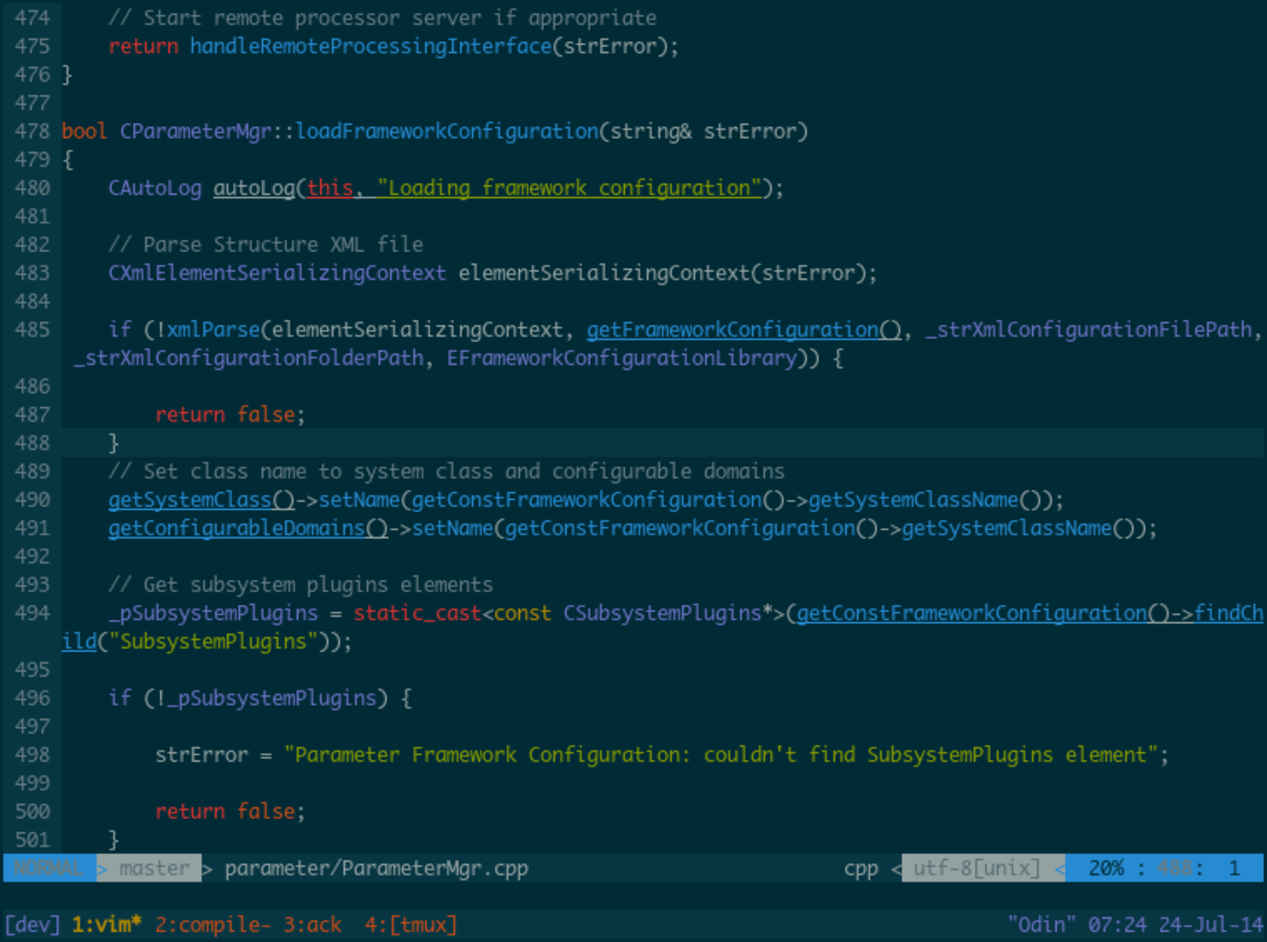
\includegraphics[width=\textwidth]{./src/img/setup.pdf}
\end{figureGraphics}

\subsection{Development}
\subsection{Verification}
\subsection{Review}
\subsection{Pre-integration}
